\section{Preliminaries}
Representation learning involves encoding an image $X \in \mathcal{X}$ to latent features $\mZ(X)$ for downstream tasks. Traditionally, vision representations take a \textit{dense} spatial form:
\[
\mZ \in \mathbb{R}^{n \times d},
\]
where $n = h \times w$ denotes the number of patches on a dense grid that partitions the image. Each grid location is represented by a feature vector $\mathbf{z}_i := \mZ_{i,:} \in \mathbb{R}^d$ for $1 \leq i \leq n$. Most vision architectures also incorporate a global representation $\mathbf{z}_0 \in \mathbb{R}^d$, typically obtained via global pooling or a specialized \texttt{[CLS]} token that undergoes self-attention with patch tokens.


Ideally, we want $\mZ$ to serve as a \textit{holistic} representation of the image $X$, which retains sufficient information about the image details, while at the same time possesses rich semantics for downstream tasks. Mathematically, we define such representation as follows:

\begin{itemize}
    \item \textbf{Reconstruction}: There exists a decoder $\mathcal{D}$ such that $\mathcal{D}(\mathbf{Z}(X)) \approx X$. This ensures the representation is spatially and texturally grounded in the physical input.
    \item \textbf{Semantics}: For a downstream task with joint distribution $(X, Y) \sim \mathcal{X} \times \mathcal{Y}$, there exists a simple predictor $f \in \mathcal{F}$ (e.g., a linear layer) such that the expected task loss $\mathbb{E}_{(X,Y)} \big[ \mathcal{L}(f(\mathbf{Z}(X)), Y) \big]$ is minimized using frozen features. Typically $Y$ reflects human perception.
\end{itemize}



Current SSL paradigms are caught in a fundamental ``\textit{Invariance Paradox}''. In order to learn high-level semantics, Joint Embedding (JE) methods (e.g. the DINO family) impose \textit{invariance} to spatial transformations, even when the image is cropped to as small as only 5\%.  On the other hand, reconstruction requires spatial detail, because every pixel shift requires a different set of features for precise reconstruction. This results in representations which are highly \textit{equivariant} to the transformation, i.e. the feature map transforms along with the transformation in the image.

Let $\mathcal{T}$ be a group of spatial transformations (e.g., translations), and $t_\theta \in \mathcal{T}$ is parametrized by $\theta$ i. A representation $\mZ (X)$ suffers from the \textit{Invariance Paradox} if it must simultaneously satisfy two contradictory constraints: 
\begin{itemize}
    \item \textbf{Semantic Invariance:} The representation should be insensitive to $t_\theta \in \mathcal{T}$: 
    \[
    \|\frac{\partial}{\partial \theta} \mZ (t_\theta \circ X)\|_F \approx 0.
    \]
    \item \textbf{Spatial Equivariance:} To allow for high-fidelity reconstruction, the representation must track spatial shifts: $\mathcal{D}(\mZ (t_\theta \circ X)) \approx t_\theta \circ X$. With chain rule and matrix norm inequalities, we have
    \[
    \|\frac{\partial}{\partial \theta}\mZ (t_\theta \circ X)\|_F \gtrsim \frac{\left\| \frac{\partial (t_\theta \circ X)}{\partial \theta} \right\|_F}{\sigma_{\max} \left( \frac{\partial \mathcal{D}}{\partial \mZ } \right)} > 0.
    \]
\end{itemize}




% In contrast, \textit{sparse visual representation} aims to represent the image with
% \[
% \mZ \in \mathbb{R}^{r \times d}, \quad r \ll h \cdot w.
% \]

% Ideally, the number of sparse tokens $r$ should be less than an order of magnitude than the total number of dense tokens $n = h\cdot w$. 
% Prior works tend to emphasize only one aspect of “representation.” For example, TiTok~\citep{yu2024image} uses 32 tokens to reconstruct an image with 256 patches at high fidelity, but its sparse features lag far behind other self-supervised vision models in semantic understanding. Conversely, MAE~\citep{he2022masked} is designed to capture semantics by reconstructing randomly masked patches, yet the resulting reconstructions are often blurry. 






\section{The STELLAR Framework}
\subsection{Sparse Image Modeling}


From now on we consider a form of representation in alternative to the dense grid-based representations describing what appears at each individual location. We start from the principle that an image depicts the physical world, which can be understood as a collection of objects located in space. 

To begin with, we model an image with a compact set of semantic concepts together with their spatial distributions. Let there be $r$ concept embeddings $\vs_1, \cdots, \vs_r \in \mathbb{R}^d$,
where each $\vs_j$ captures a distinct semantic concept. The spatial distribution of these concepts is expressed through weights $\vl_1, \cdots, \vl_n \in \mathbb{R}^{r}$, where $n$ is the total number of patches. 

By constraining $0 \leq \vl_i \leq 1$ and $\mathbf{1}^\top \vl_i = 1$, each patch is represented as a convex combination of the concept embeddings: $\vv_i = \sum_{j=1}^r \vl_{i,j} \vs_j$. Thus, the set ${\vs_j}_{j=1}^r$ acts as a basis for constructing local features. In matrix form, the latent representation now takes the form
\begin{equation}\label{eq-lowrank}
    \mZ(X) = \mL(X) \mS(X), 
\end{equation}

where
$\mS = [\vs_1, \ldots, \vs_r]^\top \in \mathbb{R}^{r \times d}$ is the \textit{semantic matrix}, and $\mL = [\vl_1, \ldots, \vl_n]^\top \in \mathbb{R}^{n \times r}$ is the \textit{localization matrix}, with the constraint $0 \leq \mL \leq 1, \mL \mathbf{1}_r =\mathbf{1}_n$.


Compared to a canonical dense representation of shape $n\times d$, $\mZ = \mL \mS$ can be considered as a form of low-rank matrix approximation from the sparse representation. While the form resembles the low-rank structure used in convex semi-nonnegative matrix factorization~\citep{ding2008convex},  $\mS$ and $\mL$ are not obtained from any matrix factorization algorithm, but are instead direct output from the forward pass of the encoder,  allowing end-to-end training  using SSL objectives.


\subsection{Equivariant Partitioning}

The factorized form in \eqref{eq-lowrank} not only provides a more efficient latent representation ($r(n+d) \ll nd$. With 16 tokens, ViT-base on a $224\times 224$ image enjoys 90\% reduction), it also provides an escape from the invariance paradox. The spatial transformation is now partitioned as follows:

\begin{equation}
    \underbrace{\frac{\partial \mZ(t_\theta \circ X)}{\partial \theta}}_{\text{Total Equivariance}} = 
    \underbrace{\left( \frac{\partial \mL(t_\theta \circ X)}{\partial \theta} \right) \mS}_{\substack{\text{Spatial Equivariance} }} + 
    \underbrace{\mL \left( \frac{\partial \mS(t_\theta \circ X)}{\partial \theta} \right)}_{\text{Semantic Variance} \approx 0}.
\label{eq:factorized_equivariance}
\end{equation}

With the spatial and semantic information disentangled, we can offload the spatial equivariance entirely to localization matrix $\mL$, while still achieving semantic invariance in $\mS$. We illustrate the learning paradigm of the factorized representation in Fig.~\ref{fig:compare}. We require that $\mZ(X)$ can reconstruct the image by minimizing 
\begin{equation}
    \mathcal{L}_{recon} = \ell(\mathcal{D}(\mL(X) \mS(X)), X).
\label{eq-recon}
\end{equation}

This \textit{low-rank approximated reconstruction} forces the model to use only sparse tokens $\{\vs_j\}_{j=1}^r$ to capture sufficient information about the image.

\begin{figure}
    \centering
    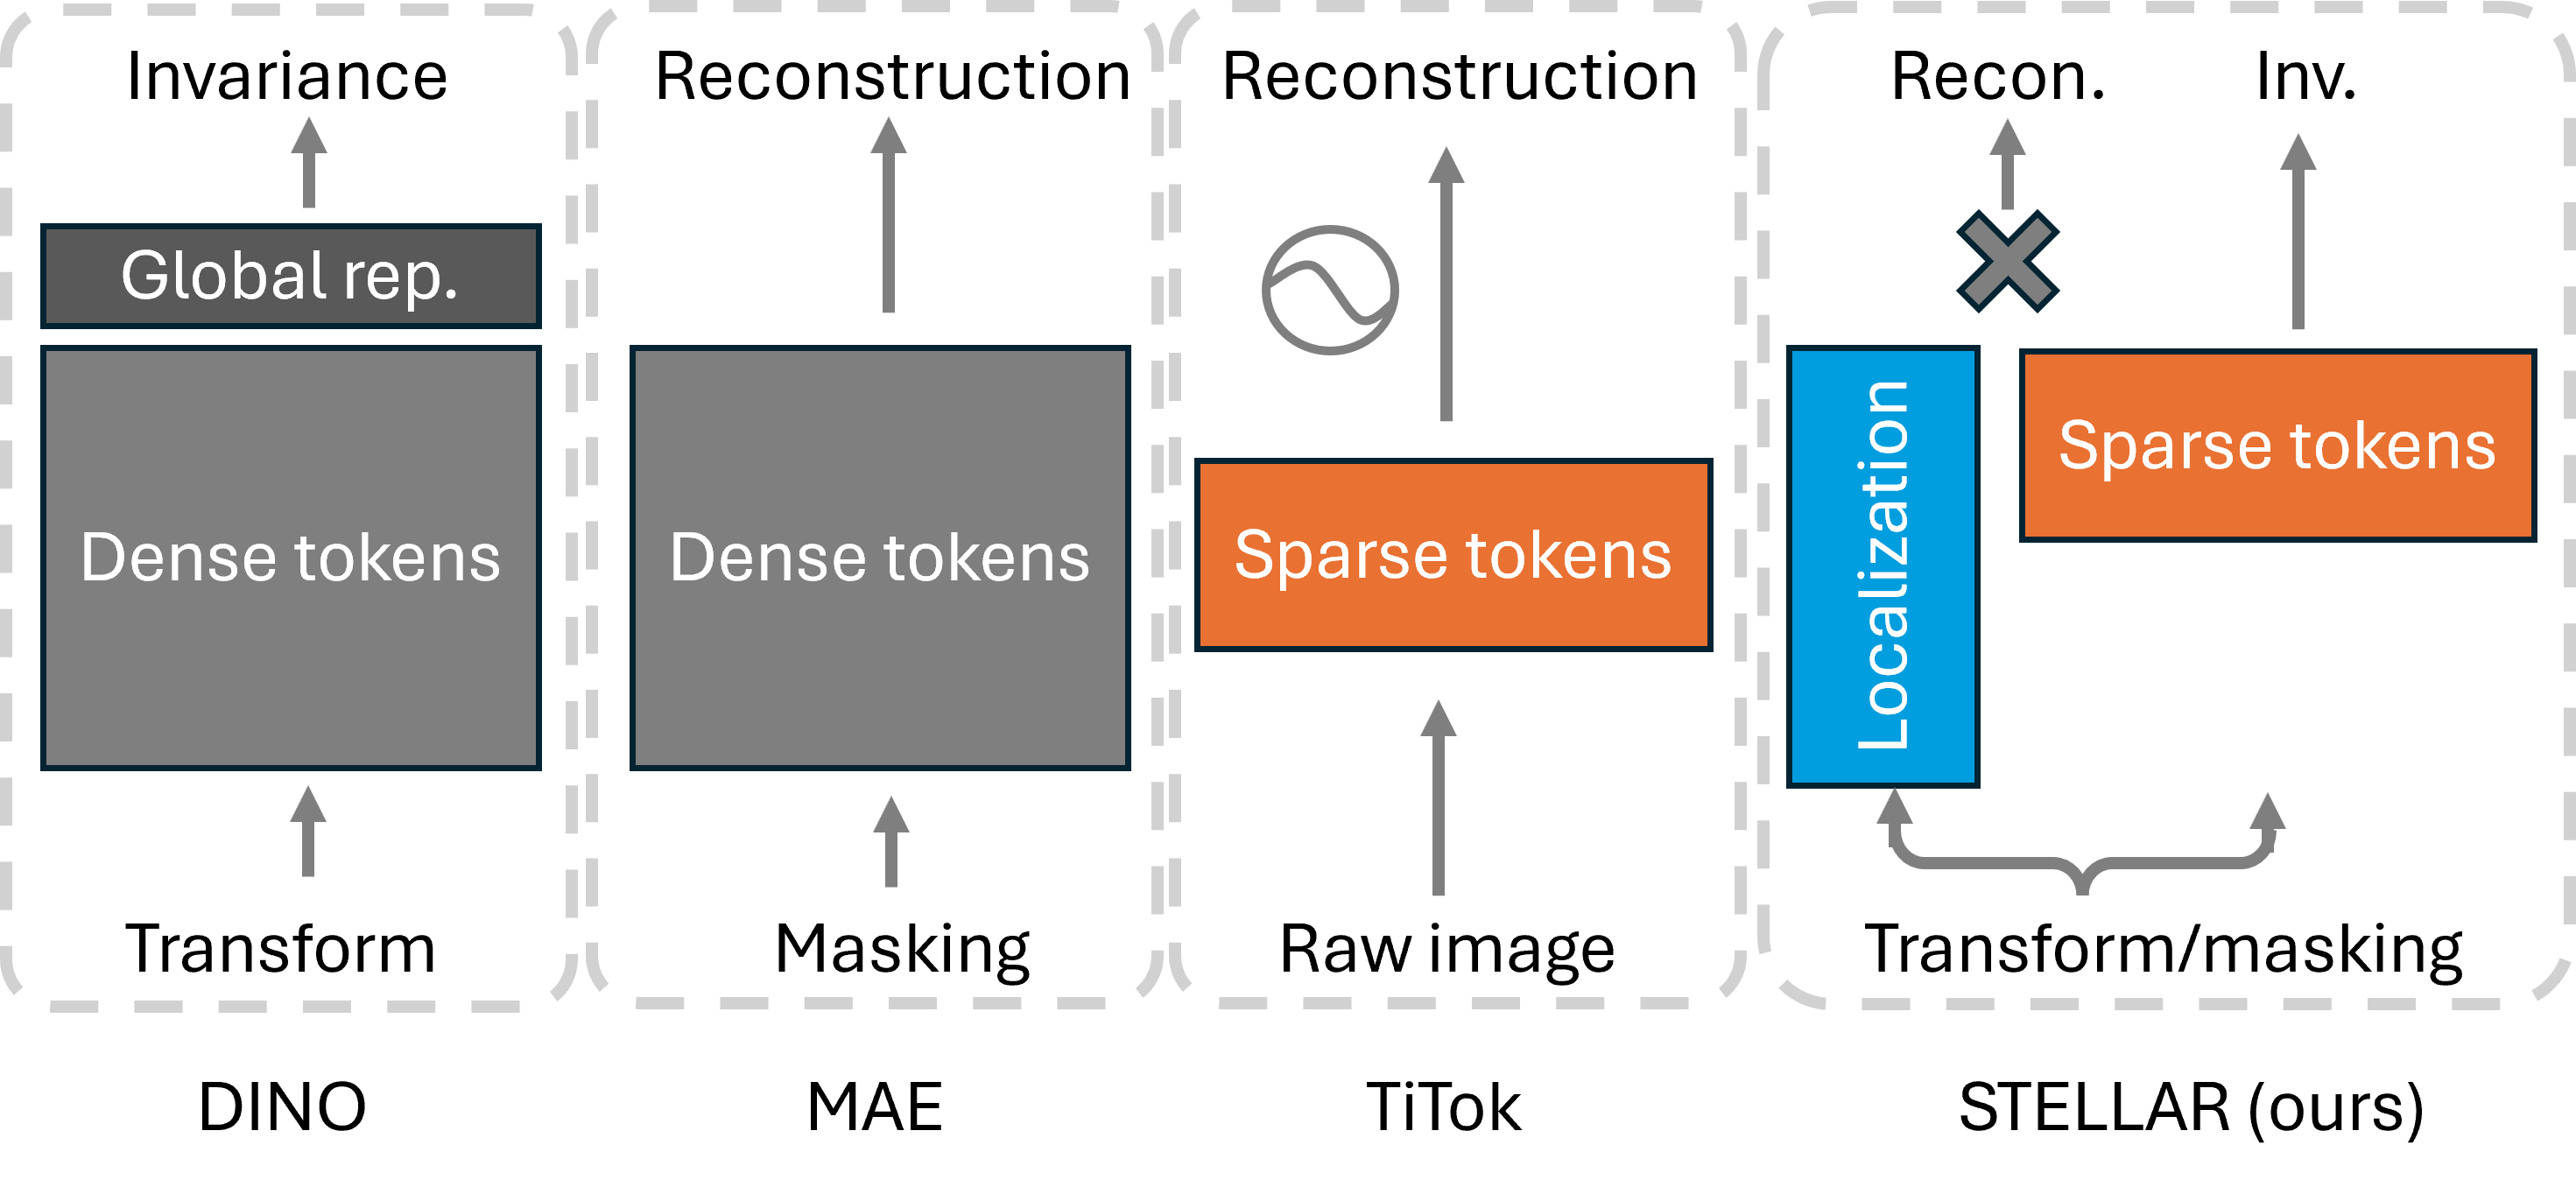
\includegraphics[width=\linewidth]{figures/Method_compare.png}
    \caption{Comparison of learning different latent representation.}
    \label{fig:compare}
\end{figure}

% Finally, a compact sparse representation is then obtained by concatenating the concept embeddings with the transposed localization matrix:
% \begin{equation}
%     \mZ = [\mS,\mL^T] \in \mathbb{R}^{r\times d^*}, \quad d^* = d + n.
% \end{equation}




\subsection{Vision Concept Clustering}\label{sec-cluster}
To encourage sparse tokens to represent transferable vision concepts, we structure them into $K$ learnable prototypes $\vc_1, \cdots, \vc_K \in \mathbb{R}^p$. A backbone encoder $\mathcal{E}$ maps a mini-batch of $m$ images into sparse features $\mS^1, \cdots, \mS^m$. Each token is projected onto the unit sphere $\mathbb{S}^{p-1}$ via a normalized projector $h: \mathbb{R}^d \rightarrow \mathbb{S}^{p-1}$, and its similarity to prototypes $\mC=[\vc_1,\cdots,\vc_K]$ gives logits
\begin{equation}\label{eq-logits}
\lambda^i_j = [\vc_1 \cdot h(\vs^i_j), \cdots, \vc_K \cdot h(\vs^i_j)], \quad j=1,\dots,r.
\end{equation}

Soft assignments over the prototypes is obtained with
\begin{equation}\label{eq-assignment}
q^i_{j,k} = \frac{\exp(\lambda^i_{j,k}/\tau)}{\sum_{k'=1}^K \exp(\lambda^i_{j,k'}/\tau)},
\end{equation}
where $\tau$ controls sharpness. Direct entropy minimization of $q^i_j$ is unstable due to non-convexity and empty clusters. Following \cite{caron2020unsupervised, darcet2025cluster}, we compute balanced assignments $\tilde{q}^i_j$ from $q^i_j$ using the Sinkhorn-Knopp algorithm (see appendix) without gradient, and minimize
\begin{equation}\label{eq-cluster}
\mathcal{L}_\text{cluster} = -\frac{1}{mr}\sum_{i=1}^m \sum_{j=1}^r \sum_{k=1}^K \tilde{q}^i_{j,k} \log q^i_{j,k}.
\end{equation}

Unlike DINOv2 and SwAV which only use Sinkhorn for balancing teacher targets, we explicitly minimize $\mathcal{L}_\text{cluster}$ along with all other objectives.

\subsection{Set Concepts Alignment}\label{sec-align}
To achieve the semantic invariance in \eqref{eq:factorized_equivariance}, we align the sparse tokens ${\vs'_1,\dots,\vs'_r}$ obtained from a transformed view (e.g. masking or cropping) to the ones from the global view ${\vs_1,\dots,\vs_r}$. However, this set concepts alignment problem is challenging compared to global representation alignment in traditional JE methods, because there is no inherent ordering in the $r$ tokens. To solve the problem, we apply optimal transport with the cost matrix
\begin{equation}
\Theta_{j'j} = \|\vs'_{j'} - \vs_j\|_2.
\end{equation}
We solve for an assignment matrix $\mP$ via entropy-regularized optimal transport:
\begin{align}\label{eq-match}
\min_{\mP \geq 0} & \quad \sum_{j',j} \mP_{j'j} \Theta_{j'j} - \epsilon H(\mP), \\
s.t. &  \quad
\mP\mathbf{1}_r = \mP^T\mathbf{1}_r = \frac{1}{r}\mathbf{1}_r,
\end{align}
with $H(\mP)=-\sum{j',j} \mP_{j'j}\log \mP_{j'j}$. We solve for $\mP$ using the Sinkhorn algorithm, and define the matching $\sigma(j') := \text{argmax}_j \mP_{j'j}$. Compared to bipartite matching algorithms such Hungarian matching widely used in previous literature, this algorithm is up to $100\times$ faster, with experimental results analyzed in the appendix.

We then compute prototype assignments for the transformed view tokens $q'_{j'} = \text{softmax}(\mC^T h(\vs'_{j'})/\tau)$, and minimize the set concept alignment loss
\begin{equation}\label{eq-align}
\mathcal{L}_\text{align} = -\frac{1}{r}\sum_{j'=1}^r \sum_{k=1}^K \tilde{q}_{\sigma(j'),k}\log q'_{j',k}.
\end{equation}

Optionally, we use the same framework to cluster and align the CLS token with its own projector and prototypes, similar to previous JE methods. However, we do not used it for reconstruction. We also apply KoLeo regularization~\citep{sablayrolles2018spreading} on the normalized sparse tokens $\bar{\vs}_j := \vs_j/\|\vs_j\|$ obtained from the same image to encourage concept diversification: 
\begin{equation}
    \mathcal{L}_{KoLeo} = -\frac{1}{r} \sum_{j=1}^r \log\left(\min_{j' \neq j} \frac{1}{2}\| \bar{\vs}_j - \bar{\vs}_{j'}\|_2 \right).
\end{equation}

All together, we jointly optimize the following objectives by training the encoder $\mathcal{E}$, decoder $\mathcal{D}$, projector $h$, and prototypes $\mC$ jointly with the final objective:
\begin{align}
\min_{\mathcal{E}, \mathcal{D}, h, \mC} \quad & a_1\mathcal{L}_\text{recon} + a_2\mathcal{L}_\text{cluster} + a_3\mathcal{L}_\text{align} + \\ & a_4\mathcal{L}_\text{cluster-cls} + a_5\mathcal{L}_\text{align-cls} + a_6\mathcal{L}_\text{KoLeo}.
\end{align}


In summary, we proposed a sparse vision representation $(\mS, \mL) = \mathcal{E}(X)$ that explicitly disentangles semantic concepts from their spatial distributions, enabling the latent variables to support both pixel-level reconstruction and high-level semantic understanding. We introduced a simple encoder design to obtain these latent variables and SSL objectives to shape them into transferable visual concepts.

We refer to our framework of learning the spatial-semantic factorized representation $\mZ(X) = \mL(X) \mS(X)$ as \textbf{S}parse \textbf{T}oken \textbf{E}xtraction and \textbf{L}ocalization with \textbf{L}ow-rank \textbf{A}pproximated \textbf{R}econstruction (STELLAR). 

\subsection{Model Design}
We note that the framework only specifies the latent space, and does not prescribe any specific encoder or decoder architecture. In this work, we adopt a simple design with common modules and model architectures to obtain $\mS$ and $\mL$ as described below.

For the encoder part, we use an existing ViT\citep{dosovitskiy2020image} as the backbone, and equip it with $r$ learnable latent query vectors, which are passed to the transformer blocks alongside the patch tokens. Processed by the ViT jointly, the latent queries produce sparse tokens $\mS \in \mathbb{R}^{r \times d}$. 

% In order to} obtain the localization matrix $\mL \in \mathbb{R}^{n \times r}$ associated with the sparse tokens, we simply project $\mS$ and $\mU$ to a shared space, and} compute pairwise cosine similarities between projected dense and sparse features, followed by a softmax normalization with temperature $t$:
% \begin{equation}
%     \mL = \text{softmax}\left(1/t \cdot \text{cossim}(\mU \mW_1, \mS \mW_2)\right),
% \end{equation}
% where $\mW_1$ and $\mW_2$ are learnable linear projections, and $t$ controls the sharpness of the spatial distribution. We note that this form is similar to the attention weights in a single head attention from the dense tokens to the sparse tokens, despite L2 normalization and dedicated softmax temperature. This simple form was proven to be effective in obtaining $\mL$ in our experiments.}

To obtain the localization matrix $\mL \in \mathbb{R}^{n \times r}$ associated with the sparse tokens, we use the dense feature map $\mU \in \mathbb{R}^{n \times d}$ output from the image patches. We project both $\mS$ and $\mU$ into a shared embedding space and compute their pairwise cosine similarities, followed by a softmax normalization with temperature $\tau_\text{spatial}$ along the the second dimension:
\begin{equation}
    \mL = \text{softmax}\left(\text{cossim}(\mU \mW_1, \mS \mW_2)/\tau_\text{spatial} \right).
\end{equation}

\begin{figure*}[!hbt]
    \centering
    
    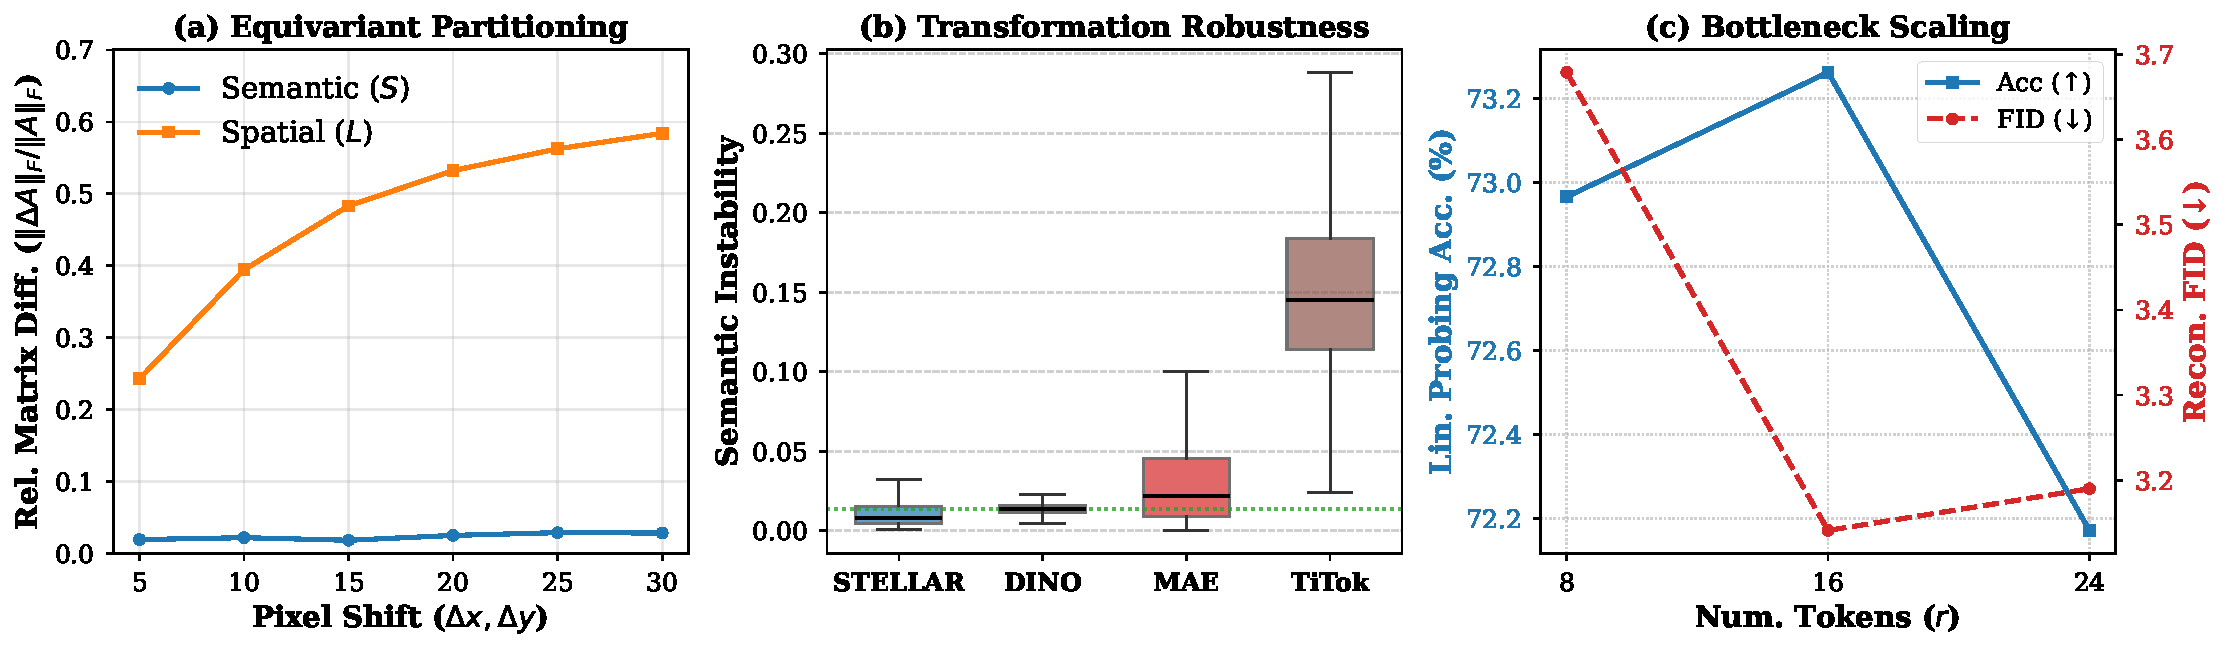
\includegraphics[width=\textwidth]{figures/stellar_main_results.pdf}
    \caption{Analysis of STELLAR representation. (a) Relative matrix difference in $\mL$ and $\mS$ under controled pixel shift in the input image. (b) Cosine distance of latent representation under random 50-100\% random cropping. (c) Impact of number of sparse tokens $r$ on reconstruciton and semantic quality.}
    \label{fig:analysis}
\end{figure*}

$\mW_1$ and $\mW_2$ are learnable linear projections, and $\tau_\text{spatial}$ controls the sharpness of the spatial distribution. We note that his mapping is structurally similar to the attention weights obtained in a single-head cross-attention layer, up to the use of L2 normalization and an explicit temperature parameter. Therefore, the latent representation  $\mZ = \mL \mS$ can be viewed as rebuilding a dense feature map for reconstruction by cross-attending to only $r$ sparse concept tokens.



All together, the encoder $\mathcal{E}$ includes ViT transformer blocks, $r$ learnable latent query vectors, and projection layers $\mW_1, \mW_2$. The decoder $\mathcal{D}$ is a 6-layer lightweight ViT reconstructing the image patches.

The STELLAR framework can be used on a pretrained ViT such as MAE or DINO to leverage the foundation prior and shape it into a sparse holistic representation. It can also be trained from a random prior and reach competitive spatial, semantic, and reconstruction quality. We provide deep analysis in the ablation study.

% Although the low-rank form $\mL \mS$ is simple, it effectively disentangles high-level semantic concepts from low-level spatial localization. This yields two key benefits for both reconstruction and representation learning:

% \begin{itemize}
% \item The concept matrix $\mS$ no longer needs to encode spatial information, and can instead focus purely on learning what objects or visual concepts are present. Through the linear combination $\mL \mS$, these concepts can be flexibly allocated across spatial locations to form a dense semantic map, enabling efficient reconstruction.

%     \item Because the semantic embeddings in $\mS$ are independent of location, we can freely apply image transformations while enforcing consistency in the learned concepts. This invariance induces robust high-level semantic features that transfer well to image understanding tasks.  

% \end{itemize}




% We cluster the sparse visual concepts from the dataset into prototypes in an online manner. Random partial views (masking, cropping) are passed to the same encoder, and aligned to the global view using set optimal transport.

% In addition, we optionally use an exponential moving average (EMA) updated momentum encoder to encode the target assignments $\tilde{q}$ in \eqref{eq-cluster} and \eqref{eq-align}. We observed that using a momentum encoder is essential in the warm-up stage when training from scratch, but suboptimal in subsequent training. We provide detailed results in ablation study. 